\documentclass[12pt]{article}
\usepackage[english]{babel}
\usepackage[utf8]{inputenc}

%% Pointer to 'default' preamble, other reusable files
% pacakages and definitions

\usepackage{geometry}
\geometry{
	letterpaper, 
	portrait, 
	top=.75in,
	left=.8in,
	right=.75in,
	bottom=.5in		} 	% Page Margins
	
%% additional packages for nice things
\usepackage{amsmath} 	% for most math
\usepackage{commath} 	% for abs
\usepackage{lastpage}	% for page count
\usepackage{amssymb} 	% for therefore
\usepackage{graphicx} 	% for image handling
\usepackage{wrapfig} 	% wrap figures
\usepackage[none]{hyphenat} % for no hyphenations
\usepackage{array} 		% for >{} column characterisctis
\usepackage{physics} 	% for easier derivative \dv....
\usepackage{tikz} 		% for graphic@!
\usepackage{circuitikz} % for circuits!
\usetikzlibrary{arrows.meta} % for loads
\usepackage[thicklines]{cancel}	% for cancels
\usepackage{xcolor}		% for color cancels
\usepackage[per-mode=fraction]{siunitx} % for si units and num
\sisetup{group-separator = {,}, group-minimum-digits = 3} % additional si unit table functionality

\usepackage{fancyhdr} 	% for header
\usepackage{comment}	% for ability to comment out large sections
\usepackage{multicol}	% for multiple columns using multicols
\usepackage[framed,numbered]{matlab-prettifier} % matlab sytle listing
\usepackage{marvosym} 	% for boltsymbol lightning
\usepackage{pdflscape} 	% for various landscape pages in portrait docs.
%\usepackage{float}
\usepackage{fancyvrb}	% for Verbatim (a tab respecting verbatim)
\usepackage{enumitem}	% for [resume] functionality of enumerate
\usepackage{spreadtab} 	% for using formulas in tables}
\usepackage{numprint}	% for number format in spread tab
\usepackage{subcaption} % for subfigures with captions
\usepackage[normalem]{ulem} % for strike through sout

% for row colors in tables....
\usepackage{color, colortbl}
\definecolor{G1}{gray}{0.9}
\definecolor{G2}{rgb}{1,0.88,1}%{gray}{0.6}
\definecolor{G3}{rgb}{0.88,1,1}

% For table formatting
\usepackage{booktabs}
\renewcommand{\arraystretch}{1.2}
\usepackage{floatrow}
\floatsetup[table]{capposition=top} % put table captions on top of tables

% Caption formating footnotesize ~ 10 pt in a 12 pt document
\usepackage[font={small}]{caption}

%% package config 
\sisetup{output-exponent-marker=\ensuremath{\mathrm{E}}} % for engineer E
\renewcommand{\CancelColor}{\color{red}}	% for color cancels
\lstset{aboveskip=2pt,belowskip=2pt} % for more compact table
%\arraycolsep=1.4pt\def
\setlength{\parindent}{0cm} % Remove indentation from paragraphs
\setlength{\columnsep}{0.5cm}
\lstset{
	style      = Matlab-editor,
	basicstyle = \ttfamily\footnotesize, % if you want to use Courier - not really used?
}
\renewcommand*{\pd}[3][]{\ensuremath{\dfrac{\partial^{#1} #2}{\partial #3}}} % for larger pd fracs
\renewcommand{\real}[1]{\mathbb{R}\left\{ #1 \right\}}	% for REAL symbol
\newcommand{\imag}[1]{\mathbb{I}\left\{ #1 \right\}}	% for IMAG symbol
\definecolor{m}{rgb}{1,0,1}	% for MATLAB matching magenta
	
%% custom macros
\newcommand\numberthis{\addtocounter{equation}{1}\tag{\theequation}} % for simple \numberthis command

\newcommand{\equal}{=} % so circuitikz can have an = in the labels
\newcolumntype{L}[1]{>{\raggedright\let\newline\\\arraybackslash\hspace{0pt}}m{#1}}
\newcolumntype{C}[1]{>{\centering\let\newline\\\arraybackslash\hspace{0pt}}m{#1}}
\newcolumntype{R}[1]{>{\raggedleft\let\newline\\\arraybackslash\hspace{0pt}}m{#1}}

%% Header
\pagestyle{fancy} % for header stuffs
\fancyhf{}
% spacing
\headheight 29 pt
\headsep 6 pt
%%% custom commands for nicer units
\newcommand{\mw}{\ensuremath{\text{ MW}}}
\newcommand{\hz}{\ensuremath{\text{ Hz}}}
\newcommand{\pu}{\ensuremath{\text{ Pu}}}
\newcommand{\sbase}{\ensuremath{\text{S}_{\text{Base}}}}
\newcommand{\fbase}{\ensuremath{f_{\text{Base}}}}
\newcommand{\mbase}[1]{\ensuremath{\text{M}_{\text{Base}_{#1}}}}
\newcommand{\hsys}{\ensuremath{\text{ H}_{\text{sys}}}}


%% Header
\rhead{Thad Haines \\ Page \thepage\ of \pageref{LastPage}}
\chead{Talking Points \\ Week of October 21th, 2019}
\lhead{Research \\ }

%\usepackage{graphicx}
%\graphicspath{ {figures/} }
%\newcommand{\caseName}{ }

\begin{document}
\begin{multicols}{2}
\raggedright
	\paragraph{Recent Progress:}
	\begin{enumerate}
\itemsep0em 
		\item Noise Agent Created

		\item Deadband Experimental Results

	%	\item More \verb|matplotlib| plot functions created.

		\item GitHub updated:\\
		\verb|https://github.com/thadhaines/|
		
	\end{enumerate}
\paragraph{Current Tasks:}
	\begin{enumerate}
		\itemsep0em 
		\item Paper for IEEE PES
		%\item Generic Governor testing
		\item Continue to refine BA ACE actions.
		%\item Update Code flowchart% to aid in further development.
		\item Thesis work 
		%\item Keep Goals and Requests in mind.
		
		%\subitem A FlowtabrDAO exists that can find flow between busses. A way to initialize bus connections between areas has yet to be devised.

	\end{enumerate}

	\paragraph{Current Questions:}
	\begin{enumerate}
\itemsep0em 
	\item Realistic AGC results and/or tuning?
	\item Typical deadbands of AGC? 
	\item IEEE Paper outline or title?\\Long-Term Effect of Governor Deadband on Valve Travel
	\end{enumerate}
	
\paragraph{Deadband Explained} \ \\
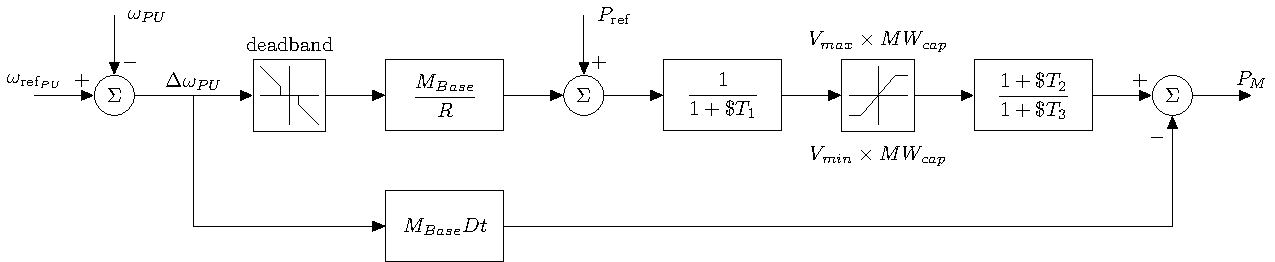
\includegraphics[width=\linewidth]{tgov1DB}\\
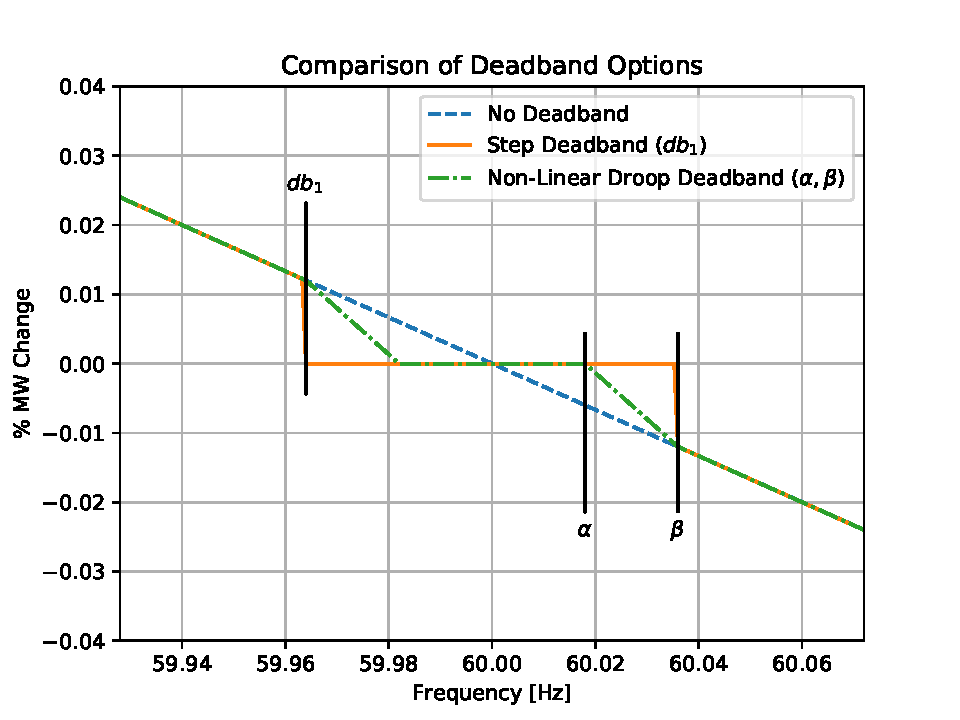
\includegraphics[width=\linewidth]{dbAction2}

\paragraph{MiniWECC AGC Settings}

\begin{itemize}
\itemsep0em 
\item 15 second ACG Action Time
\item PI filtered ACE
\item 15 Second Windowed IACE included
\item Step Deadband at 36 mHz
\item N-L Droop from 16-36 mHz
\end{itemize}
\vfill\null
\columnbreak
\paragraph{MiniWECC Noise Results} \ \\
System Loading (0.05\% Noise Added):\\
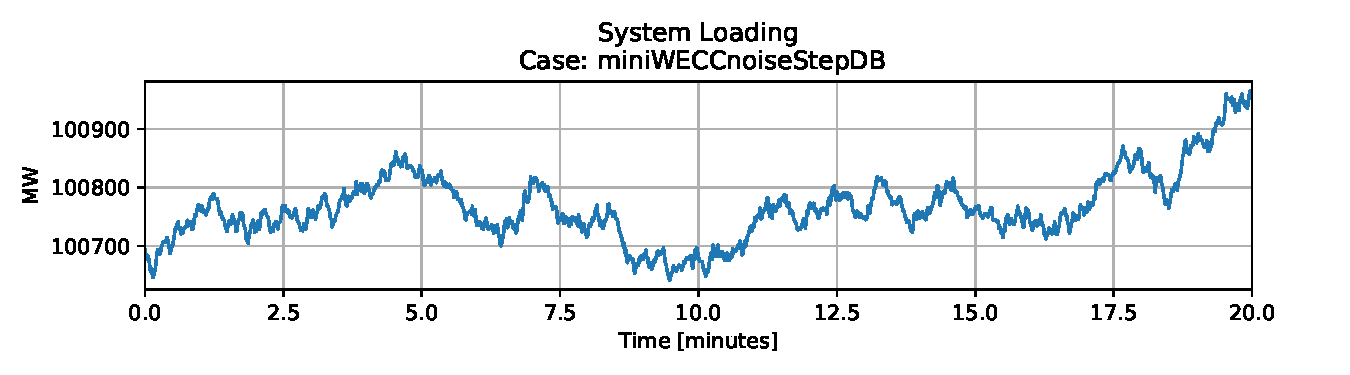
\includegraphics[width=\linewidth]{miniWECCnoiseStepDBPload}
Step DB:\\
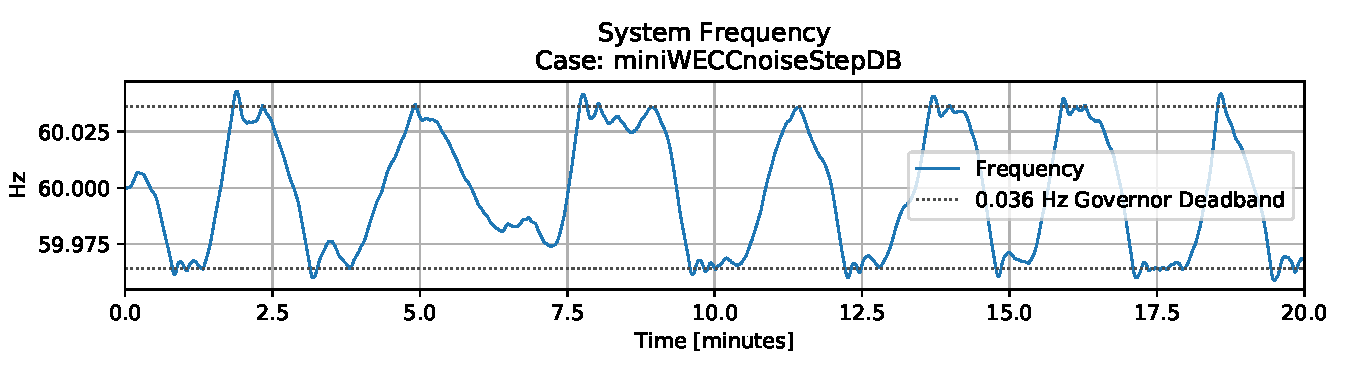
\includegraphics[width=\linewidth]{miniWECCnoiseStepDBFreq}
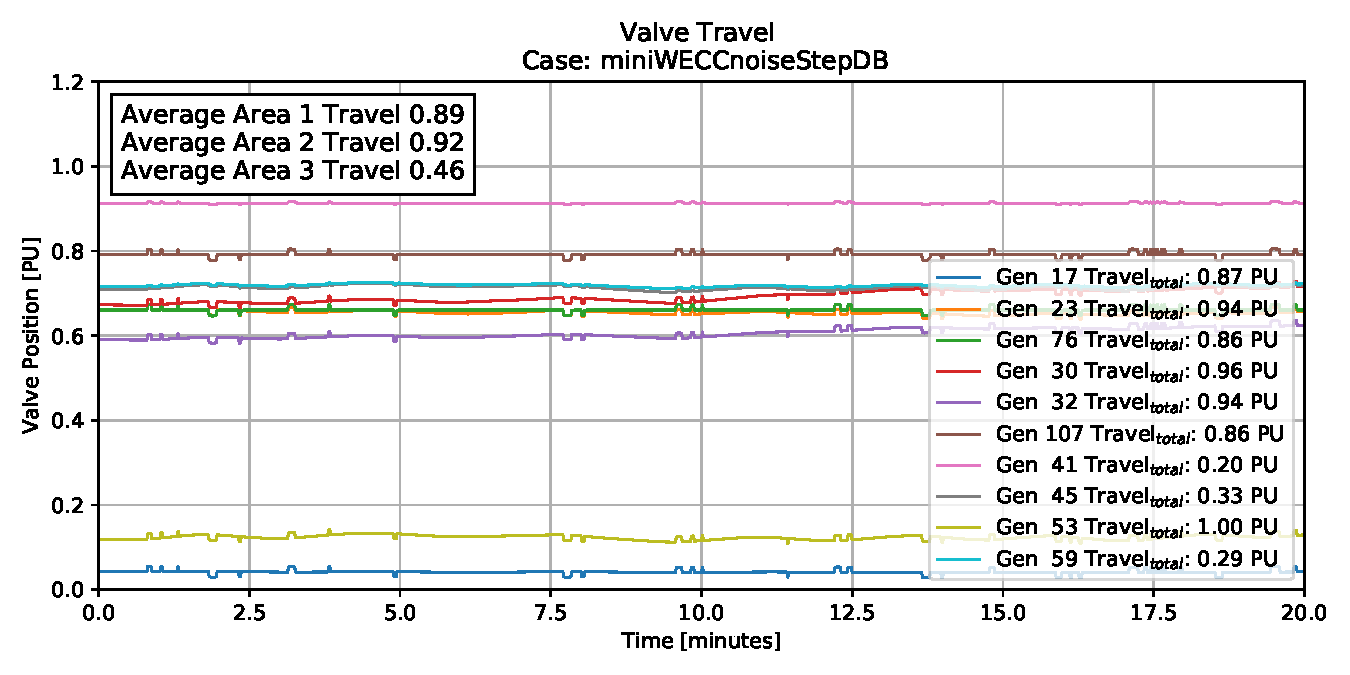
\includegraphics[width=\linewidth]{miniWECCnoiseStepDBValveTravel01}
Non-linear Droop DB:\\
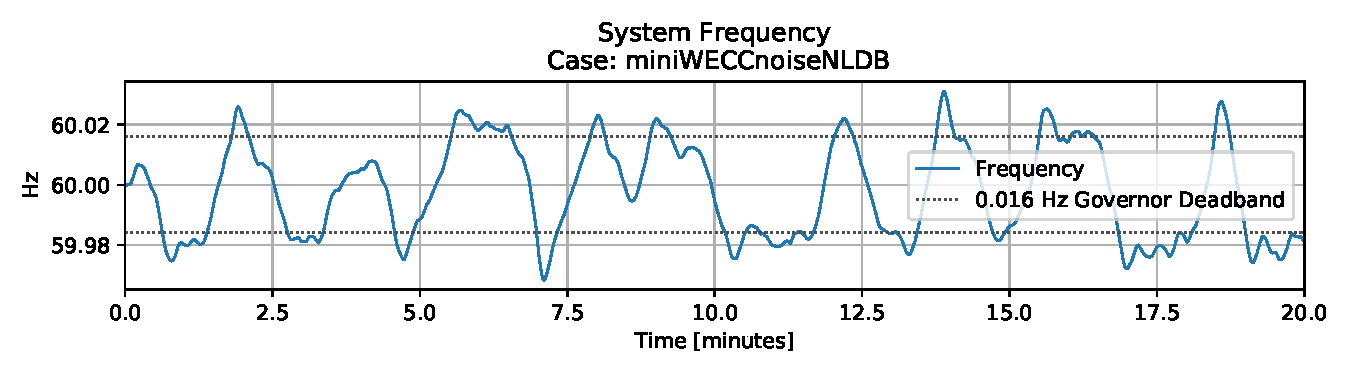
\includegraphics[width=\linewidth]{miniWECCnoiseNLDBFreq}
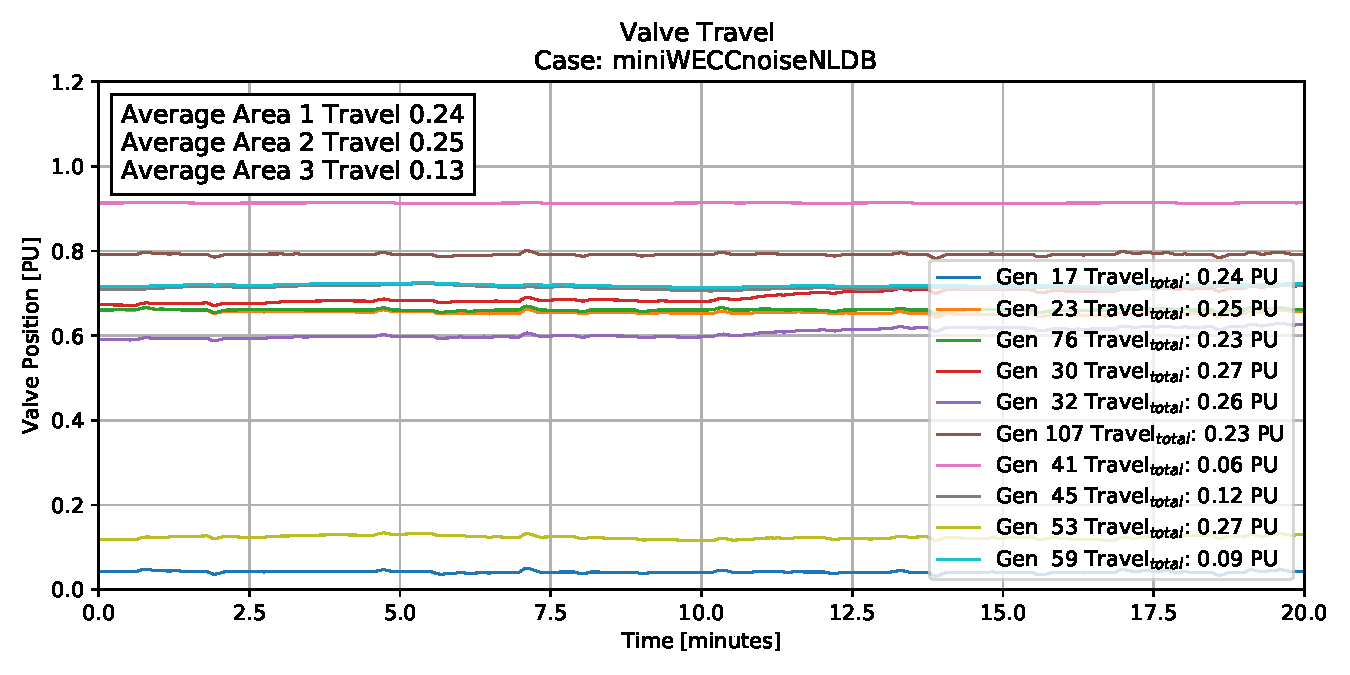
\includegraphics[width=\linewidth]{miniWECCnoiseNLDBValveTravel01}
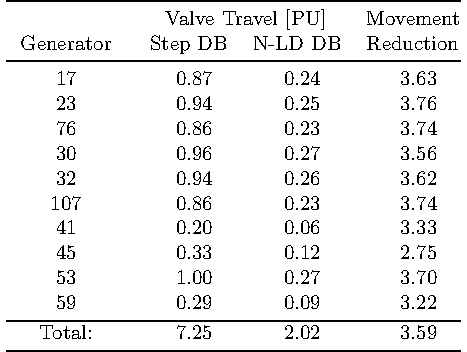
\includegraphics[width=.9\linewidth]{miniWECCnoiseRes01}

\vfill\null
\end{multicols}
%\pagebreak
\paragraph{AGC Block Diagram} \ \\

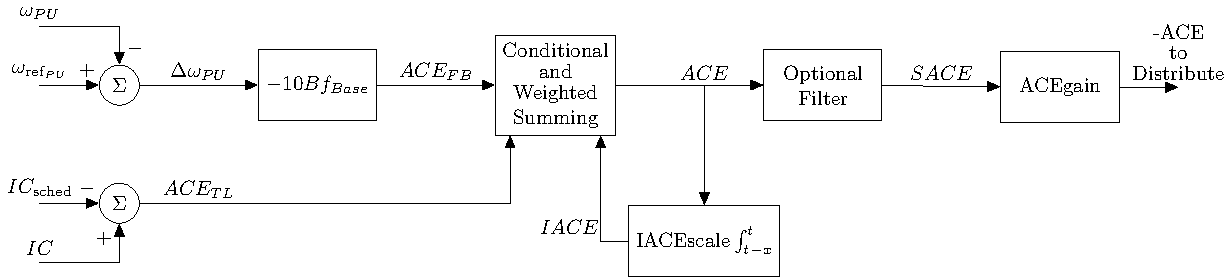
\includegraphics[width=\linewidth]{AGC-TLB}\\
Optional Filters:\\
\begin{center}
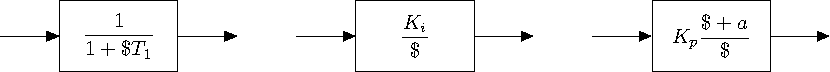
\includegraphics[width=.8\linewidth]{filterAgent}
\end{center}

\paragraph{Controller Results (no noise)} miniWECC 1500 MW generation loss at t=2\ \\
No Deadband:\\
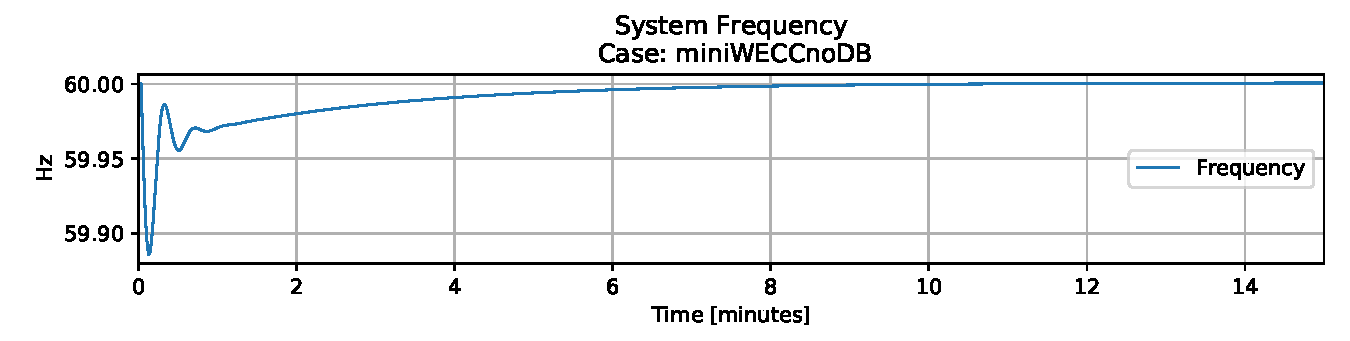
\includegraphics[width=\linewidth]{noDB}
{Step Deadband:\\
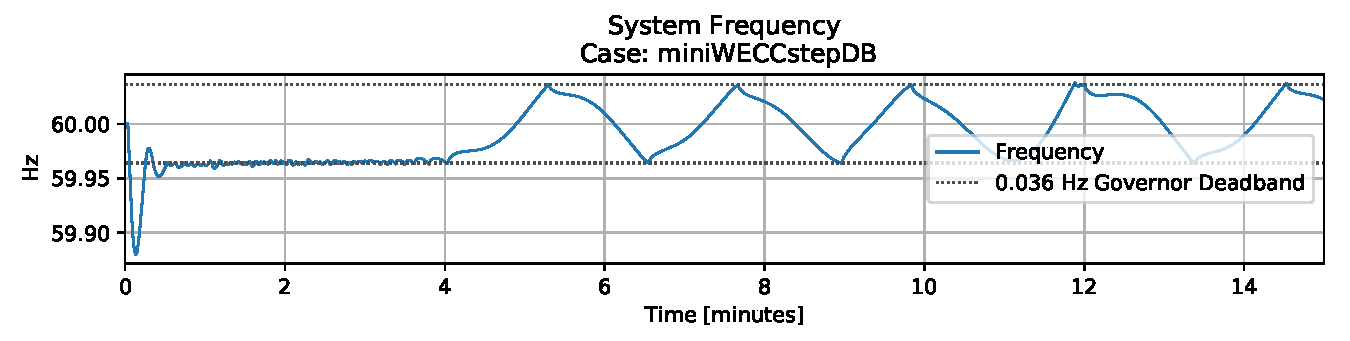
\includegraphics[width=\linewidth]{stepDB}
Non-Linear Droop:\\
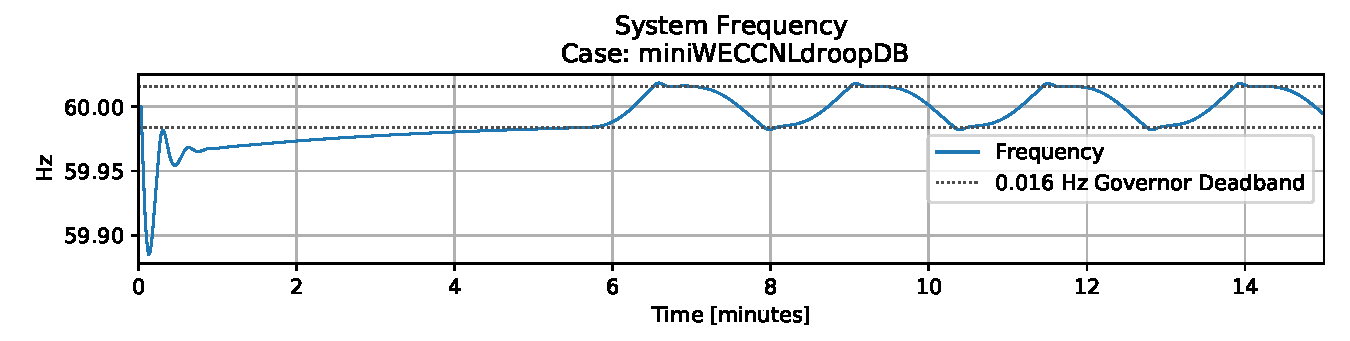
\includegraphics[width=\linewidth]{NLdroopDB}
\begin{comment}
% Common 2nd col removed 

\paragraph{Future Tasks:} %(Little to No Progress since last time / Things coming down the pipe)
	\begin{enumerate}
		
		\item Add import mirror / bypass mirror init sequence option to prevent repeated mirror creations.

		\item Bring wind into simulation \\ (ramp ungoverned generators?)

		\item Find best/correct way to trip gens in PSLF from python.

		\item Investigate line current data.
		
	\end{enumerate}
\paragraph{Future Work: (not by me)}
\begin{itemize}
\item Account for different types of loads. (exponential load model) % read from dyd
\item Work to incorporate Matt's \emph{Suggested Use Cases} into simulation.
		\begin{itemize}
		\item Add Shunt Group Agent
		\item Work to Define Definite Time Controller user input
		\end{itemize} 


		\item Investigate ULTC action.

		\item Create an agent for every object: \\ ULTC, SVD, Transformer, \ldots

		\item Get away from reliance on GE
		
\end{itemize}

\paragraph{Matt Requests:}
\begin{enumerate}
		\item Enable multiple dyd files to overwrite / replace previously defined agents/parameters
		\item Allow for variable time steps.
\end{enumerate}

	\end{enumerate}


\pagebreak
\end{comment}


%\paragraph{'Soft Goals':}
%	\begin{enumerate}
%	\item Write Thesis 2020
%	\end{enumerate}
		

\begin{comment}

\end{comment}

\end{document}